\section{Modifier un poste client}Par ce dialogue, vous pouvez modifier la configuration d'un poste client. A part des champs de saisie que vous connaissez d\'ej\`a du dialogue d'ajout d'un poste client, il y a trois colonnes o\`u vous pouvez indiquer ce qui se doit passer avec les valeurs y entr\'ees.\\
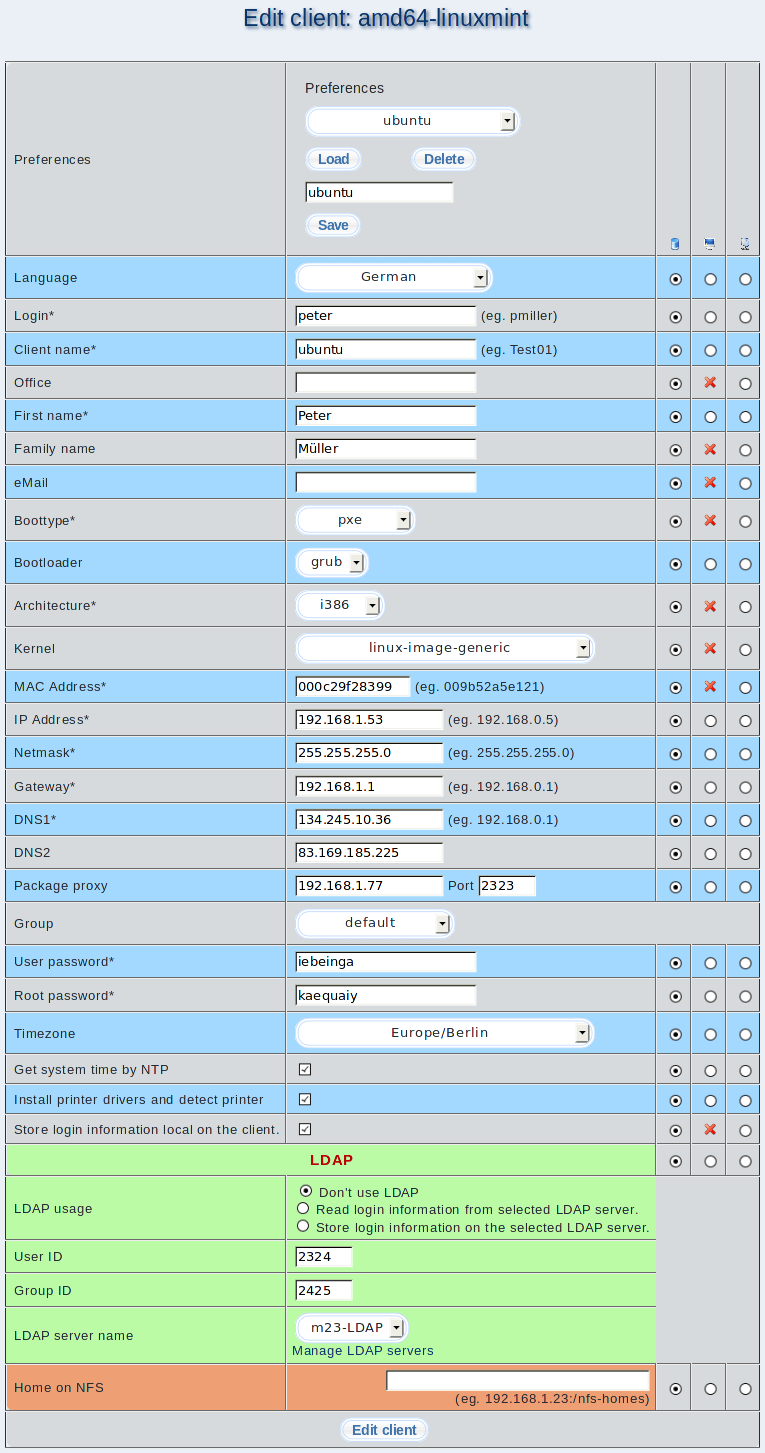
\includegraphics[scale=0.4]{/mdk/doc/manual/screenshots/fr/edit_client.png} \\
\begin{itemize}
\item \textbf{Colonne gauche}: Si vous s\'electionnez cette colonne, la valeur enregistr\'ee sur le poste client et le serveur restera inchang\'ee.\\
\item \textbf{Colonne au milieu}: Les changements doivent \^etre ex\'ecut\'es sur le poste client et apr\`es, les donn\'ees sur le serveur seront actualis\'ees.\\
\item \textbf{Colonne droite}: Seul les valeurs dans la banque de donn\'ees sur le serveur seront chang\'ees. Ceci est utile, par exemple, quand les changements sur le poste client ont d\'ej\`a \'et\'es ex\'ecut\'es \`a la main.\\
\end{itemize}
\subsection{Notez}
Certaines configurations seront enregistr\'ees seulement sur le serveur. Pour cette raison, une modification sur le poste client n'est pas possible. La colonne au milieu ne peut pas \^etre s\'electionn\'ee pour ces configurations.\\
